% =====================================================================
% The component-differential residual in the omega Cen proper-motion
% dispersion profile: a pre-registered campaign that cannot identify
% its mechanism.
% Tim Swanson -- The Omega Centauri Society / Post Oak Labs
% Build: pdflatex axi-note && bibtex axi-note && pdflatex x2
% BUILDER DRAFT (WU OCS-AXI-NOTE-1). Version line owned by the editorial
% session; leave \date at "Draft v0.5 (last revised 2026-08-27)".
%
% Plan of record: paper/AXI-PREREGISTRATION.md (ADOPTED 2026-08-14),
%   including amendments AXI-A1, AXI-A2, AXI-A3 and the Campaign closure
%   section. Every quotable / not-quotable line there is binding here.
% Sources of record:
%   paper/axi/stage0/STAGE0_REPORT.md        (stage 0)
%   paper/axi/stage1/GATES_REPORT.md         (X-G-f, X-G-a, n=1600 extension)
%   paper/axi/stage1/M1_FIT_REPORT.md        (M1 fit, X-G-b, X-G-c, X-G-d)
%   OCS-REFEREE-G-AXI-ROUND_2026-08-14.md    (Aarons adopt-after-changes)
%   OCS-REFEREE-AXI-X2_2026-08-15.md         (Aarons/Okafor/VM on X-G-a)
% Figure data: paper/axi/stage1/fit_results/m1_fit_results.json
%   (rows m1_td*_plummer_5494, reading "joint MAP"), redrawn as pgfplots.
% =====================================================================
\documentclass[11pt]{article}

\usepackage[margin=1.1in]{geometry}
\usepackage{newtxtext,newtxmath}
\usepackage[round,authoryear]{natbib}
\usepackage{graphicx}
\usepackage{booktabs}
\usepackage{amsmath}
\usepackage{tikz}
\usepackage{pgfplots}
\pgfplotsset{compat=1.17}
\usepgfplotslibrary{fillbetween}
\usepackage[font=small,labelfont=bf]{caption}
\usepackage{microtype}
\usepackage[colorlinks=true,linkcolor=blue!50!black,citecolor=blue!50!black,urlcolor=blue!50!black]{hyperref}
\usepackage{xcolor}

\newcommand{\msun}{\ensuremath{M_\odot}}
\newcommand{\ocen}{$\omega$~Cen}
\newcommand{\as}{\ensuremath{^{\prime\prime}}}
\newcommand{\dD}{\ensuremath{\delta_D}}
\newcommand{\dS}{\ensuremath{\delta_S}}
\newcommand{\tD}{\ensuremath{\tau_D}}
\newcommand{\specbox}[1]{\par\smallskip\noindent\fbox{\parbox{0.97\linewidth}{\small\textbf{Epistemic status:} #1}}\smallskip\par}

\title{\textbf{The Component-Differential Residual in the Omega Centauri Proper-Motion Dispersion Profile: A Pre-Registered Campaign That Cannot Identify Its Mechanism}}
\author{Tim Swanson\\[2pt]
\small The Omega Centauri Society / Post Oak Labs\\
\small \texttt{tim@postoaklabs.com}}
\date{August 2026 \\[4pt] \small Draft v0.5 (last revised 2026-08-27) --- methods note for the AXI campaign;\\ \small companion to the mass-tension paper (Paper H); prepared for omegacentauri.me}

\begin{document}
\maketitle

\begin{abstract}
\noindent
A fit of the oMEGACat proper-motion dispersion profile of \ocen{} under a shared smooth discrepancy in the mean leaves a component-differential residual: the model under-predicts the sky-radial dispersion and over-predicts the sky-tangential one, coherently, at every radius and every reading of the grid \citep{HFit2Report2026}. This note records a campaign pre-registered to identify the mechanism behind that residual \citep{AXIPrereg2026}, run to its stopping rule, and closed on its own pre-registered outcome that no mechanism can be named. Four hypotheses were specified in advance with separating discriminants: anisotropy structure beyond one Osipkov-Merritt scale (H-A), flattening with azimuthal averaging (H-B), unrelaxed accretion-origin substructure (H-C), and component-dependent measurement systematics (H-D). Stage 0 could run two of the four on the frozen radial table, and both discriminants failed at all twelve residual-evaluation points; H-B and H-C were not tested. Stage 1 fitted M1, a component-resolved discrepancy model that decomposes the shared spline into a shared term \dS{} and a differential term \dD{} on the same four knots. M1 clears the per-component adequacy test the shared model failed, at all 36 readings, with a minimum $p$ of 0.0301 over 144 tests. Two other gates go against it. Cross-axis stability fails on one of five pre-committed statements, through a discrete switch between the differential and the white systematic term that moves with the \dD{} prior width; and the budget check fires, because the differential the profile leg requires exceeds twice its equipartition-derived budget beyond about $130\as$, by up to a factor of 3.8. Under the pre-registered consequence clauses this makes decision criterion~4, ``the campaign cannot identify the mechanism'', the only quotable outcome. The measured object that survives is the \dD{} amplitude, 0.16 to 0.45~km\,s$^{-1}$ over 36 readings, positive everywhere and inside the calibrated region everywhere, with a median split of 0.29 to 0.33~km\,s$^{-1}$ inside the knot span against the 0.27 to 0.31~km\,s$^{-1}$ that stage 0 measured independently. Escalation to an axisymmetric model is forbidden by the budget gate's own clause. Paper H is untouched throughout.
\end{abstract}

\bigskip
\noindent\textbf{Keywords:} globular clusters: individual: NGC 5139 (Omega Centauri); stars: kinematics and dynamics; proper motions; methods: statistical

\specbox{This is a methods record of a pre-registered campaign that reached a pre-registered negative outcome. Nothing here is a mechanism claim, and nothing here is a claim about the cluster's dark component. The one measured quantity offered for quotation is the \dD{} amplitude, which is quotable only inside the calibrated region of Section~\ref{sec:gates-a} and travels with the two gate failures of Section~\ref{sec:outcome}.}

\section{Question and plan}
\label{sec:question}

Paper H's A2 amendment replaced every quadrature floor on the profile leg with a smooth discrepancy in the mean, a four-knot cubic spline $\delta(r)$ in $\log_{10} r$ with knots at $\{5, 20, 80, 300\}\as$, shared by both proper-motion components, in the framework of \citet{KennedyOHagan2001}. The FIT-2 record measured what that model leaves behind \citep{HFit2Report2026}. Runs tests on the standardised profile residuals pass everywhere, at $p = 0.24$ to $0.98$. The sign tests do not: 31 to 34 of 40 sky-radial residuals are positive, at $p = 4.2\times10^{-5}$ to $8.4\times10^{-6}$, while the sky-tangential component is over-predicted in 25 to 29 of 40 bins. The verdict is identical at all three cell readings and in all twelve profile-leg configurations.

A shared $\delta(r)$ cannot represent a residual of that shape, and the marginalisation over a single Osipkov-Merritt anisotropy scale, $r_a \in \{1.5, 3, 6, 15, \infty\}$~pc, does not absorb it either. The object is a coherent split between the two sky components at every radius. The campaign recorded here was pre-registered to ask which named mechanism produces it \citep{AXIPrereg2026}.

\subsection{Scope, fixed before any fit}
\label{sec:scope}

The pre-registration carries a mandatory disclosure into every report the campaign produces, and it is reproduced here once, in its own words:

\begin{quote}
This campaign improves the visible model and may open the inner bins. The outer profile does not arbitrate compact-versus-extended under any version of it.
\end{quote}

The boundary comes from a radius-resolved terminality ruling on Paper H's profile leg. Beyond about $50\as$ the systematics budget runs 10 to 40 times the statistical errors, and those radii carry less than $10^{-3}$ of the dark component's enclosed-mass signal, so the bins that dominate the leg carry no verdict signal. Per the terminality ruling, a better error model does not create signal the geometry does not put there.

The boundary permits, narrowly: the inner bins ($\lesssim 10\as$), where signal-to-systematics is of order unity, are marginal rather than terminal, and a campaign that closed the component-differential residual there might make them usable. That route runs through decision criterion~5 of the plan and needs its own ratified amendment to Paper H's pre-registration. It forbids, by pre-commitment: no re-scoring of Paper H's criteria 2, 3 or 4 from this campaign's output, no restoration of the profile leg to the configuration that Paper H's own misspecification gate dropped, and no relaxation of Paper H's standing embargo list. This note makes no statement of any kind about the cluster's dark component, and it quotes no dark-component posterior.

\subsection{Four hypotheses, with their separating discriminants}
\label{sec:hypotheses}

\begin{description}
\item[H-A, anisotropy structure beyond one Osipkov-Merritt scale.] The true $\beta(r)$ is not in the one-parameter family the visible model carries, and the mismatch shows as a component-differential residual because $\beta$ enters $\sigma_R$ and $\sigma_T$ with opposite sign. Signature: the split tracks the gradient of the measured anisotropy profile rather than the local dispersion amplitude \citep{Zocchi2017,Zocchi2019,Aros2020}.
\item[H-B, flattening with azimuthal averaging.] A spherical model fitted to azimuthally averaged data of a flattened system ($\epsilon = 0.17$, \citealt{WhiteShawl1987}, the largest published value; star-count isophotes give 0.11--0.12 with a rounder core, \citealt{Geyer1983,Pancino2003}) produces a component-differential residual by construction. Signature: this campaign takes residual power at $\cos 2\phi$ in position angle as the diagnostic for this mechanism, with the split amplitude scaling as the flattening of the axisymmetric models in \citep{vanderMarelAnderson2010}.
\item[H-C, unrelaxed substructure of accretion origin.] \ocen{} is the stripped nucleus of an accreted system, and the split is the imprint of a subpopulation that has not phase-mixed \citep{Ibata2019,BekkiTsujimoto2019,Clontz2024}. Signature: a patchy split differing between subsamples at the same radius, the one signature of the four that separates subsamples of the same catalogue.
\item[H-D, component-dependent measurement systematics.] The split is in the catalogue rather than in the cluster: residual distortion or a per-epoch orientation imbalance projects unequally onto the two sky directions once they are defined relative to the cluster centre \citep{Haberle2024oMEGACatII,Haberle2025oMEGACatVI}. Signature: organisation on detector or epoch geometry and on per-bin star counts rather than on cluster-centric radius. Confirming H-D would end the campaign rather than extend the model, so it was tested first.
\end{description}

Decision criterion~2 names a hypothesis as identified only when its own discriminant passes and the other three fail on theirs. Criterion~4 records in advance that ``the campaign cannot identify the mechanism'' is an acceptable and publishable outcome, to be stated as such if criterion~2 names no hypothesis in at least half the defined cells.

\subsection{Data and gates}
\label{sec:data-gates}

The data are frozen at listed versions: the 40 adaptive log bins of the oMEGACat VI dispersion and anisotropy table, $r = 1.8209$ to $311.1198\as$ over 610{,}846 stars, undigitised, with its asymmetric sky-radial and sky-tangential errors \citep{Haberle2025oMEGACatVI}; the visible-model pair carried as a reported bracket with neither member promoted, a Plummer sphere at the \citet{BaumgardtHilker2018} half-light scale and the $\alpha\beta\gamma$ profile of \citet{BanaresHernandez2025}; and both distances, 5494 and 5200~pc. The line-of-sight rotation table \citep{Haberle2026LVM} is a line-of-sight observable and enters no likelihood at any stage. No fast-star data and no pulsar data enter the campaign, so both legs of Paper H's verdict configuration are untouched by construction.

Six gates were fixed before any fit, each with its consequence clause: X-G-a, injection and recovery at the real per-bin error level with component-differential misspecification injections including a sign-flipped member; X-G-b, per-component sign and runs tests at $p > 0.01$ in all four tests at all three readings; X-G-c, cross-axis stability of every reported statement across both visible models, both distances and the halved and doubled \dD{} prior rows; X-G-d, a budget check that fires if the required differential exceeds twice its named budget anywhere inside the knot span; X-G-e, a standing scope gate with no statistic, checked by the referee panel; and X-G-f, a pre-real-data check that M1 at $\dD \equiv 0$ reproduces the shared-discrepancy fit to the recorded digit. Section~4.3 of the plan opens with the rule that all gates must pass before any statement from the campaign is quotable.

\section{Stage 0: the two discriminants the frozen table can carry}
\label{sec:stage0}

Stage 0 was diagnostic only, with no new likelihood, run against the existing residuals at the three residual-evaluation points crossed with both visible models and both distances \citep{AXIStage0Report2026}. Its thresholds were committed and dated in the deliverable before any discriminant statistic was computed. The primary statistic is the per-bin split $D_i = e_{R,i} - e_{T,i}$, from which the shared $\delta(r)$ cancels by construction, so it is independent of the shared-term posterior.

Two of the four hypotheses cannot be tested on the frozen radial table at all. H-B needs a position-angle-resolved dispersion field and H-C needs per-star population assignments, and neither is in the table. Stage 0 therefore recorded in advance that it cannot name any hypothesis as identified whatever its statistics return, because two of the three required failures are unavailable. H-B and H-C are not tested and are nowhere called disfavoured.

\paragraph{H-A: FAIL.} The correlation of the split with the anisotropy gradient runs $|\rho| = 0.081$ to $0.185$ at $p = 0.248$ to $0.614$, against a committed threshold of $|\rho| \geq 0.40$ at $p < 0.01$ at all twelve readings. The signature condition, that the split track the anisotropy gradient more strongly than the dispersion amplitude, holds at none of the twelve. The verdict is stable at all three smoothing bandwidths.

\paragraph{H-D: FAIL.} The correlation with per-bin star counts runs $|\rho| = 0.144$ to $0.233$ at $p = 0.147$ to $0.370$, and its radius-controlled partial runs 0.082 to 0.145 against a threshold of 0.30. The surface-density form of the predictor behaves the same way. The committed stop-or-continue rule stops the campaign only on a passing H-D discriminant, so it did not fire.

\paragraph{What the table cannot separate.} The three predictors and radius are close to the same variable in rank space over the frozen 40 bins: the anisotropy gradient correlates with radius at $\rho = -0.986$ at the primary bandwidth and at $-1.000$ at the widest, star counts with radius at $+0.986$, and dispersion with radius at $-0.970$. An uncontrolled rank correlation with any of them is close to a rank correlation with radius, which is why the partial-correlation controls were committed in advance and why both hypotheses fail those controls on the secondary standardised statistic while passing the raw correlation. This is a measurement-design fact about the azimuthally averaged table rather than a finding about the cluster.

\paragraph{The scale check.} The one component-differential effect measured in the same catalogue is the energy-equipartition asymmetry, $\eta = 0.088 \pm 0.017$ at the centre falling to $0.049 \pm 0.009$ at the half-light radius over the mass range 0.288 to 0.690~\msun{}, with the radial component of equipartition declining much faster with radius than the tangential \citep{Haberle2025oMEGACatVI}. Against the predicted differential scale $\Delta_{\rm pred} = \sigma\,\eta\,\tfrac12 \ln(m_{\max}/m_{\min})$, the observed median $|D|$ of 0.52 to 0.53~km\,s$^{-1}$ gives a ratio of 0.724 to 0.735 at every reading, inside the committed consistency band of $[0.5, 2.0]$. The median signed split is $+0.27$ to $+0.31$~km\,s$^{-1}$, with the sky-radial component as the under-predicted one, reproducing the direction of the FIT-2 record. The comparison carries no verdict for any hypothesis and was committed as a check on the prior derivation of Section~\ref{sec:m1}.

\section{Stage 1: the M1 model and the gate battery}
\label{sec:m1}

M1 is the minimal extension of the shared discrepancy model, in the same framework. The shared mean discrepancy is decomposed on the same four knots,
\begin{align}
\sigma_{R,\rm model}(r) &\rightarrow \sigma_{R,\rm model}(r) + \dS(r) + \dD(r), \\
\sigma_{T,\rm model}(r) &\rightarrow \sigma_{T,\rm model}(r) + \dS(r) - \dD(r),
\end{align}
with \dS{} keeping the existing Normal$(0, 1.0\ {\rm km\,s^{-1}})$ independent knot priors, the half-Normal$(0, 0.3\ {\rm km\,s^{-1}})$ white systematic $s$ retained unchanged, and both terms marginalised in every reported quantity. M1 reduces to the shared model exactly at $\dD \equiv 0$. It adds four nuisance dimensions and no new physics machinery, and by construction it measures the differential rather than explaining it.

The \dD{} knot prior is Normal$(0, 0.5\ {\rm km\,s^{-1}})$, derived before any fit as the upper edge of the equipartition-differential term from the frozen $\eta$ profile rather than as half of the shared budget. Flattening is excluded from that scale. The halved and doubled prior rows, $\tD \in \{0.25, 0.5, 1.0\}$~km\,s$^{-1}$, are mandatory and were noted non-trivial in advance, on the precedent that halving the shared model's knot prior had flipped evidence signs across whole configurations.

\subsection{X-G-f, the pre-real-data reproduction check: PASS}
\label{sec:gates-f}

Against the artifact the gate originally named, the check failed: log-evidence moved by 0.065 to 0.291 nats in all 16 configurations. The traced cause is not M1. The profile leg is the only object M1 changes, and the M1 profile-leg likelihood cube reproduces the reference to $0.000\times10^{0}$ nats in all 16 configurations, with the whole discrepancy sitting in the acceleration leg, which the campaign does not touch, and accounted for by a reconciliation of the two pulsar spatial distributions committed one day after the reference was recorded \citep{AXIGatesReport2026}. No code in the repository could reproduce the superseded kernel, so the gate as written tested a property of its reference. Amendment AXI-A1 repointed it to the same driver re-executed under the reconciled kernel, against which the same run reproduces every scalar, every posterior array, every log-likelihood cube, all 288 prior cells and the gate record to $0.000\times10^{0}$. No code and no number changed between the failure and the pass.

\subsection{X-G-a, injection and recovery: FAIL, with a calibrated region}
\label{sec:gates-a}

Nine signed members were run at $n = 400$ mock realisations each: a point-mass injection, an extended injection, and a null, each carrying a coherent component-differential misspecification at $+0.5$, $+1.0$ and $-0.5$~km\,s$^{-1}$. Five of the nine fail a committed threshold, in two modes that separate cleanly \citep{AXIGatesReport2026}.

\paragraph{Mode 1, the amplitude interval.} Empirical two-sided 90\,per~cent interval coverage of the \dD{} amplitude is 0.8500 to 0.8775 at an injected $\pm0.5$~km\,s$^{-1}$, inside the required $[0.85, 0.95]$, and 0.7125 to 0.7200 at $+1.0$~km\,s$^{-1}$ in every injection, with Wilson intervals reaching only 0.755 to 0.762. The measured cause is a 7 to 8\,per~cent multiplicative shrinkage of the amplitude from the knot prior, against an interval width that does not grow to match it.

\paragraph{Mode 2, inherited coverage.} Coverage of the injected dark component under the extended injection sits at 0.8425 to 0.8475 at $n = 400$, below the band with Wilson intervals containing it. Amendment AXI-A2 authorised one pre-committed extension of the three extended members to $n = 1600$ on a continued seed stream, committed and dated before it was run, with the verdict scored on the pooled sample whatever it returned and no second extension permitted. It resolves below the band: 0.8237 to 0.8325 pooled, with Wilson upper limits of 0.8416, 0.8452 and 0.8500. The coverage curve reproduces to about 0.01 at every nominal level the compression measured for the shared model before any differential block existed \citep{HCalReport2026}, and it is constant along the differential axis, so this is an inherited property of the profile leg rather than an effect of \dD{}. The campaign quotes no dark-component posterior, so the consequence attaches to criterion~5, which stays closed.

\paragraph{What passes.} The null member manufactures no evidence at any differential, with median $|\ln K| = 0.16$ to $0.18$ against a threshold of~1 and a breach fraction of at most 0.0025. Correct-sign recovery is 400 of 400 in both signal injections, and the sign-flipped member added at referee request recovers at least as well as its mirror, symmetric to 0.025.

\paragraph{The regional ruling.} Under AXI-A2 the amplitude axis is scored regionally. \dD{} amplitudes are quotable only inside the calibrated region $|\dD| \leq 0.5$~km\,s$^{-1}$, where all six $\pm0.5$ members pass; the $+1.0$ members remain failed and mark the boundary. Any amplitude outside the region is reported with the measured calibration attached, a bias of about $-8$\,per~cent of amplitude and an interval about 15\,per~cent narrow at 1.0~km\,s$^{-1}$, and is not quotable as a measurement. Every \dD{} figure carries the region boundary, and the doubled-prior row is reported alongside the primary as the shrinkage sensitivity check.

\subsection{X-G-b, the adequacy gate the shared model failed: PASS}
\label{sec:gates-b}

Twelve fits were run, the four primary configurations crossed with the three \dD{} prior rows, each read at the three residual-evaluation points, for 36 readings and 144 tests. The fit driver and the gate scorer were committed unexecuted before the first fit ran, so neither gate is scored on a statement list chosen after the numbers were seen \citep{AXIFitReport2026}.

\begin{table}[htbp]
\centering
\small
\caption{The per-component adequacy tests, M1 against the shared discrepancy model on the same 40 bins. Both models pass every runs test; the sign test is where they differ.}
\label{tab:xgb}
\begin{tabular}{lll}
\toprule
statistic & shared model (A2) & M1 \\
\midrule
sign test, sky-radial & 31 to 34 of 40 positive & 20 to 25 of 40 positive \\
sign test, sky-radial, $p$ & $4.2\times10^{-5}$ to $8.4\times10^{-6}$ & 0.154 to 1.000 \\
sign test, sky-tangential & 25 to 29 of 40 over-predicted & 19 to 26 of 40 positive \\
sign test, sky-tangential, $p$ & failing at every reading & 0.0807 to 1.000 \\
runs tests, both components & 0.24 to 0.98 & 0.0301 to 0.932 \\
minimum $p$ at any reading & sign test, $8.4\times10^{-6}$ & runs test, 0.0301 \\
readings passing & 0 of 12 configurations & 36 of 36 readings \\
\bottomrule
\end{tabular}
\end{table}

\textbf{X-G-b: PASS}, at all 36 readings, with a minimum $p$ of 0.0301 over the 144 tests (Table~\ref{tab:xgb}). The tightest value anywhere in the battery is now a runs test rather than a sign test. The profile-leg best cell is where a sceptic should look, because the joint MAP is chosen by a different leg, and M1 passes there as well.

One qualification travels with the pass. Clearing the adequacy gate says the residual is absorbed rather than explained, because a discrepancy term absorbs component-differential signal by construction, as the plan's own description of M1 states in advance. The pass is evidence that the differential axis was the missing degree of freedom, and not evidence about which mechanism supplies it.

\subsection{X-G-c, cross-axis stability: FAIL, with the mechanism measured}
\label{sec:gates-c}

Five statements were fixed in the committed scorer: the X-G-b verdict; whether any bin inside the knot span has a \dD{} interval excluding zero, and with which sign; the X-G-d verdict; whether the maximum $|\dD|$ inside the span lies inside the calibrated region; and the sign of the amplitude with whether its interval excludes zero. Four hold across all twelve rows. The fourth does not, so \textbf{X-G-c: FAIL}.

In the eight rows at $\tD = 0.5$ and $1.0$~km\,s$^{-1}$ the maximum $|\dD|$ inside the span is 1.140 to 1.151~km\,s$^{-1}$ at all three readings, outside the region. In the four rows at $\tD = 0.25$~km\,s$^{-1}$ the readings disagree with each other: the posterior-mean and joint-MAP cells give 0.335 to 0.426~km\,s$^{-1}$, inside the region, while the profile-leg best cell gives 1.140 to 1.144, outside it.

Read per cell, this is the two-mode signature directly: at the halved prior the posterior-mean and joint-MAP cells sample the low mode (inside the calibrated region) while the profile-leg best cell samples the high mode (outside it); at the primary and doubled priors every reading samples the high mode. The per-row, per-reading classification is in this note's released record companion (\texttt{calc7/axi\_calc7\_switch.json}); no mechanism statement follows from it.

\begin{table}[htbp]
\centering
\small
\caption{The switch behind the X-G-c failure, at the fiducial-bracket MAP cell, Plummer at 5494~pc. Each row is unimodal in the white systematic $s$; the preferred solution switches between rows. Prior shrinkage cannot produce the move, because the outermost knot carries a posterior standard deviation of 0.022 to 0.042~km\,s$^{-1}$. The two right-hand columns are different objects: the bin-grid maximum is evaluated over the forty catalogue bins inside $[5, 300]\as$ (the gate convention; the $300\as$ knot is not a bin), while the outer-knot column is the spline's posterior mean at the $300\as$ knot itself. Both are correctly computed; an earlier version of this table carried only the knot value under a single ``outer knot \dD{}'' heading, where \S\ref{sec:gates-c}'s text separately quotes the bin-grid maximum. The ``mass at $s<0.06$'' column is computed directly from the posterior samples; the \texttt{s\_edge\_mass} field released alongside this note is a separate grid-edge tail-mass check ($10^{-52}$ to $10^{-57}$ in every reading) and is not this divider.}
\label{tab:switch}
\resizebox{\textwidth}{!}{%
\begin{tabular}{lrrrrr}
\toprule
$\tD$ [km\,s$^{-1}$] & $s$ mode & $s$ median & mass at $s < 0.06$ & bin-grid max, in span [km\,s$^{-1}$] & outer knot, posterior mean [km\,s$^{-1}$] \\
\midrule
0.25 & 0.09 & 0.090 & 0.034 & 0.344 & $0.354 \pm 0.042$ \\
0.50 & 0.03 & 0.030 & 0.968 & 1.145 & $1.207 \pm 0.026$ \\
1.00 & 0.03 & 0.030 & 0.969 & 1.147 & $1.209 \pm 0.026$ \\
\bottomrule
\end{tabular}%
}
\end{table}

The mechanism is a degeneracy between \dD{} and the white systematic $s$, and it is measured rather than inferred (Table~\ref{tab:switch}). The outer bins carry a component split that the fit must assign to one term or the other. At $\tD = 0.5$ or $1.0$ the fit assigns the split to a large differential and a small white systematic; at $\tD = 0.25$ it assigns the split instead to a white systematic three times larger, with inflated errors. The switch is discrete and it lands between 0.25 and 0.5.

The pre-registration recorded before any fit that the shared model had replaced one assumption controlling the verdict with another, that a component-resolved discrepancy adds a third, and that X-G-c exists to make prior-width control visible if it occurs. It occurred, X-G-c detected it, and it is reported as the anticipated mechanism rather than as an anomaly. The failure is confined to one statement, so what it removes is the ability to say where the differential sits at the outer radii, which is the region the scope boundary already places outside arbitration.

\subsection{X-G-d, the budget check: FIRES}
\label{sec:gates-d}

The gate was scored two ways, both fixed before the run: against the constant 0.5~km\,s$^{-1}$ scale named for the \dD{} prior, and against the radius-dependent equipartition band it was derived from. It fires if either is exceeded by more than a factor of two anywhere inside the knot span $[5, 300]\as$; the two bins outside the span, where the spline is a linear extrapolation, are excluded from the verdict.

The maximum $|\dD|$ inside the span runs 0.335 to 1.151~km\,s$^{-1}$ over the 36 readings, at $280.9\as$ in every one of them. Twenty-nine of the 36 readings exceed twice the constant scale, and the same 29 exceed twice the equipartition band, with a maximum ratio to the band of 1.10 to 3.77. \textbf{X-G-d: the clause FIRES.} The seven readings that do not fire are the large-$s$ solutions of Section~\ref{sec:gates-c}, so the two gate outcomes have one mechanism between them.

The consequence is applied as written: the component-differential model is declared misspecified beyond this campaign's scope, and the campaign does not escalate to an axisymmetric model on the strength of it. The excess is confined to large radius. Beyond about $130\as$ the required differential exceeds twice its budget, by up to a factor of 3.8 at the outermost bins inside the span, while inside $50\as$ it sits at 0.04 to 0.26~km\,s$^{-1}$ against a budget of 0.72 to 0.80. A four-knot spline that has to reach 1.2~km\,s$^{-1}$ at $300\as$ is absorbing something other than the equipartition asymmetry it was scaled against, at radii where the systematics budget is an order of magnitude above the statistical errors. That is a misspecification statement about M1 at large radius, and under Section~\ref{sec:scope} it is not a statement about the dark component.

\section{Outcome: criterion 4}
\label{sec:outcome}

Three of the six gates stand against escalation and none stands for it. X-G-c's consequence clause makes criterion~4 the only quotable outcome, X-G-d's clause forbids escalation to an axisymmetric model, and X-G-a stood failed with its regional licence before the real-data fit began. The campaign's outcome is therefore \textbf{criterion~4, the pre-registered ``the campaign cannot identify the mechanism''}, reported with the mechanism of the X-G-c failure named, as the clause requires. Criterion~2 is not scored: two of its four discriminants cannot be run on the frozen radial table, and nothing in stage 1 adds either. H-B and H-C remain not tested.

The outcome carries two parts, both already recorded earlier in this note. The first is the plain failure-to-identify: on the frozen radial table, H-A and H-D fail their committed discriminants at all twelve readings (\S\ref{sec:stage0}), and H-B and H-C cannot be run on that table at all. The second is the structural reason a positive result was never available from this table alone: the anisotropy gradient and the star-count predictor are rank-collinear with cluster-centric radius, $|\rho| = 0.86$ to $1.00$ across the bandwidths tested (\S\ref{sec:stage0}, ``What the table cannot separate''; \citep{AXIStage0Report2026}), so an azimuthally averaged radial table cannot separate either testable discriminant from a radius trend by construction. Neither statement adds a mechanism claim or a compact-versus-extended statement; both restate \S\ref{sec:stage0}.

\subsection{The measured object}
\label{sec:measured}

\begin{figure}[htbp]
\centering
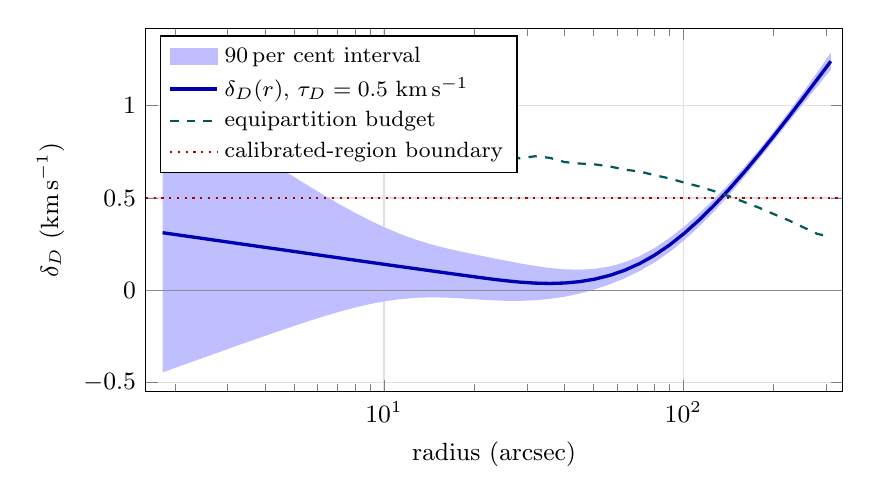
\begin{tikzpicture}
\begin{semilogxaxis}[
  width=0.86\linewidth, height=6.2cm,
  xlabel={radius (arcsec)}, ylabel={$\delta_D$ (km\,s$^{-1}$)},
  xmin=1.6, xmax=340, ymin=-0.55, ymax=1.42,
  legend style={font=\footnotesize, at={(0.02,0.98)}, anchor=north west, cells={anchor=west}},
  grid=major, grid style={black!12},
  tick label style={font=\small}, label style={font=\small},
]
\addplot[name path=lo, draw=none, forget plot] coordinates {
(1.8209,-0.4446) (3.3314,-0.2920) (4.2395,-0.2328) (5.0020,-0.1932) (5.6596,-0.1645) (6.3605,-0.1386)
(7.1334,-0.1148) (8.0028,-0.0932) (9.0465,-0.0733) (10.0358,-0.0596) (11.2893,-0.0479) (12.6994,-0.0407)
(14.2564,-0.0380) (16.0050,-0.0392) (18.0263,-0.0433) (20.1609,-0.0484) (22.6231,-0.0533) (25.2796,-0.0565)
(28.4307,-0.0570) (31.9497,-0.0538) (35.8085,-0.0464) (40.1694,-0.0343) (45.0417,-0.0173) (50.5848,0.0051)
(56.6966,0.0322) (63.5780,0.0649) (71.4233,0.1044) (80.0865,0.1509) (89.9260,0.2072) (100.7330,0.2716)
(112.9718,0.3454) (126.7619,0.4277) (142.4270,0.5182) (160.1054,0.6148) (179.1059,0.7112) (201.1505,0.8130)
(225.5429,0.9139) (252.3572,1.0127) (280.9448,1.1066) (311.1198,1.1955)};
\addplot[name path=hi, draw=none, forget plot] coordinates {
(1.8209,1.0692) (3.3314,0.7951) (4.2395,0.6874) (5.0020,0.6145) (5.6596,0.5610) (6.3605,0.5116)
(7.1334,0.4648) (8.0028,0.4202) (9.0465,0.3758) (10.0358,0.3414) (11.2893,0.3064) (12.6994,0.2760)
(14.2564,0.2508) (16.0050,0.2294) (18.0263,0.2106) (20.1609,0.1943) (22.6231,0.1777) (25.2796,0.1621)
(28.4307,0.1462) (31.9497,0.1322) (35.8085,0.1211) (40.1694,0.1137) (45.0417,0.1117) (50.5848,0.1163)
(56.6966,0.1291) (63.5780,0.1515) (71.4233,0.1851) (80.0865,0.2289) (89.9260,0.2836) (100.7330,0.3460)
(112.9718,0.4166) (126.7619,0.4941) (142.4270,0.5788) (160.1054,0.6697) (179.1059,0.7623) (201.1505,0.8640)
(225.5429,0.9697) (252.3572,1.0780) (280.9448,1.1841) (311.1198,1.2864)};
\addplot[blue!25] fill between[of=lo and hi];
\addlegendentry{90\,per~cent interval}
\addplot[blue!70!black, very thick] coordinates {
(1.8209,0.3123) (3.3314,0.2515) (4.2395,0.2273) (5.0020,0.2107) (5.6596,0.1982) (6.3605,0.1865)
(7.1334,0.1750) (8.0028,0.1635) (9.0465,0.1512) (10.0358,0.1409) (11.2893,0.1293) (12.6994,0.1177)
(14.2564,0.1064) (16.0050,0.0951) (18.0263,0.0837) (20.1609,0.0729) (22.6231,0.0622) (25.2796,0.0528)
(28.4307,0.0446) (31.9497,0.0392) (35.8085,0.0373) (40.1694,0.0397) (45.0417,0.0472) (50.5848,0.0607)
(56.6966,0.0807) (63.5780,0.1082) (71.4233,0.1448) (80.0865,0.1899) (89.9260,0.2454) (100.7330,0.3088)
(112.9718,0.3810) (126.7619,0.4609) (142.4270,0.5485) (160.1054,0.6423) (179.1059,0.7368) (201.1505,0.8385)
(225.5429,0.9418) (252.3572,1.0453) (280.9448,1.1454) (311.1198,1.2409)};
\addlegendentry{$\delta_D(r)$, $\tau_D = 0.5$~km\,s$^{-1}$}
\addplot[teal!70!black, thick, dashed] coordinates {
(1.8209,0.7974) (3.3314,0.8240) (4.2395,0.8004) (5.0020,0.8852) (5.6596,0.8511) (6.3605,0.8216)
(7.1334,0.7602) (8.0028,0.7806) (9.0465,0.7593) (10.0358,0.7860) (11.2893,0.7538) (12.6994,0.7534)
(14.2564,0.7651) (16.0050,0.7582) (18.0263,0.7570) (20.1609,0.7529) (22.6231,0.7304) (25.2796,0.7383)
(28.4307,0.7149) (31.9497,0.7264) (35.8085,0.7178) (40.1694,0.6948) (45.0417,0.6870) (50.5848,0.6823)
(56.6966,0.6717) (63.5780,0.6539) (71.4233,0.6439) (80.0865,0.6242) (89.9260,0.6063) (100.7330,0.5836)
(112.9718,0.5628) (126.7619,0.5373) (142.4270,0.5095) (160.1054,0.4779) (179.1059,0.4477) (201.1505,0.4124)
(225.5429,0.3785) (252.3572,0.3408) (280.9448,0.3054) (311.1198,0.2900)};
\addlegendentry{equipartition budget}
\addplot[red!70!black, thick, dotted] coordinates {(1.6,0.5) (340,0.5)};
\addlegendentry{calibrated-region boundary}
\addplot[black!45, thin, forget plot] coordinates {(1.6,0) (340,0)};
\end{semilogxaxis}
\end{tikzpicture}
\caption{The primary output, criterion~1: the \dD{} posterior against radius at the primary prior row, Plummer at 5494~pc, fiducial bracket, read at the joint MAP as a residual-evaluation point. The other eleven rows and the other two brackets differ in the third decimal except where Section~\ref{sec:gates-c} says otherwise. The curve crosses the calibrated-region boundary at about $130\as$, and \textbf{the pointwise curve beyond that crossing is outside the calibrated region and is not quotable as a measurement} (Section~\ref{sec:gates-a}). Values from \texttt{fit\_results/m1\_fit\_results.json}.}
\label{fig:deltaD}
\end{figure}

The \dD{} amplitude, defined as the injection gate defined it, runs 0.159 to 0.447~km\,s$^{-1}$ over the 36 readings, positive everywhere, with the 90\,per~cent interval excluding zero everywhere. Every value sits inside the calibrated region, so no amplitude reported here needs the out-of-region calibration attached. The pointwise curve is a different matter (Figure~\ref{fig:deltaD}): $\dD(r)$ crosses the region boundary at about $130\as$ and reaches 1.15~km\,s$^{-1}$ at $280.9\as$, so the outer half of the curve is outside the calibrated region, is drawn with the boundary marked, and is not quotable as a measurement. The regional calibration was measured on the amplitude rather than on the pointwise curve, which is a limitation of the calibration and is stated as one.

Two regimes separate in the posterior width. Inside about $50\as$ the posterior standard deviation is 0.054 to 0.187~km\,s$^{-1}$, of order the prior scale, so the inner differential is prior-dominated and the data barely constrain it. Beyond about $100\as$ it falls to 0.018 to 0.019~km\,s$^{-1}$, twenty to fifty times smaller, with the posterior at 0.5 to 1.0~km\,s$^{-1}$. The differential the profile leg requires is concentrated at the radii the terminality ruling of Section~\ref{sec:scope} already places behind a systematics floor 10 to 40 times the statistical errors. The inner-region statement here is about the width of a prior-dominated posterior and is not an inner-bin usability claim, which routes through criterion~5 alone.

\paragraph{The untuned external check.} Stage 0 measured the split $D = e_R - e_T$ at a median of $+0.27$ to $+0.31$~km\,s$^{-1}$ before M1 existed, and M1 parameterises that split as $2\dD$. Over the twelve primary-row readings the fitted median $2\dD$ inside the knot span is $+0.291$ to $+0.334$~km\,s$^{-1}$, recovering the stage-0 split to about 5\,per~cent with no part of the pipeline tuned to make it do so. The ratio to the budget does not carry across as cleanly: on the absolute statistic stage 0 used, the median $|2\dD|$ over the median budget is 0.41 to 0.47 here against 0.72 to 0.74 there. Stage 0 took the absolute value of a noisy per-bin residual, which inflates its median, while M1's \dD{} is a spline that has already smoothed that noise away. The signed medians, which are not subject to that inflation, agree.

\begin{figure}[htbp]
\centering
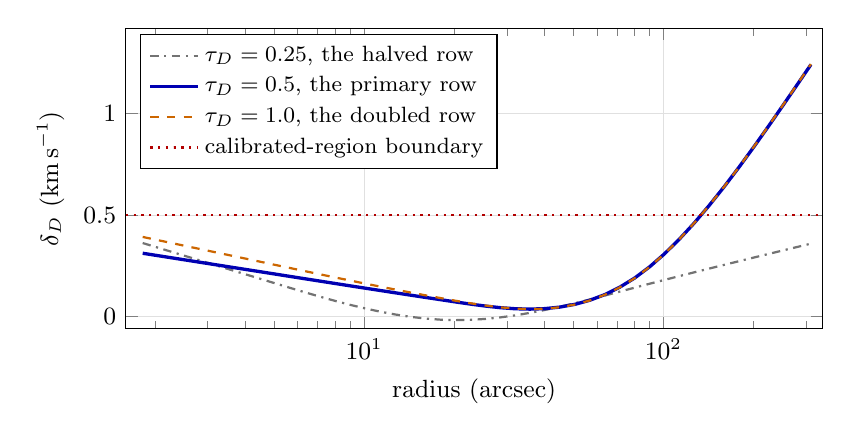
\begin{tikzpicture}
\begin{semilogxaxis}[
  width=0.86\linewidth, height=5.4cm,
  xlabel={radius (arcsec)}, ylabel={$\delta_D$ (km\,s$^{-1}$)},
  xmin=1.6, xmax=340, ymin=-0.06, ymax=1.42,
  legend style={font=\footnotesize, at={(0.02,0.98)}, anchor=north west, cells={anchor=west}},
  grid=major, grid style={black!12},
  tick label style={font=\small}, label style={font=\small},
]
\addplot[black!55, thick, dashdotted] coordinates {
(1.8209,0.3626) (3.3314,0.2450) (4.2395,0.1981) (5.0020,0.1659) (5.6596,0.1419) (6.3605,0.1196)
(7.1334,0.0983) (8.0028,0.0778) (9.0465,0.0573) (10.0358,0.0414) (11.2893,0.0251) (12.6994,0.0110)
(14.2564,-0.0004) (16.0050,-0.0090) (18.0263,-0.0147) (20.1609,-0.0169) (22.6231,-0.0156) (25.2796,-0.0112)
(28.4307,-0.0037) (31.9497,0.0065) (35.8085,0.0188) (40.1694,0.0331) (45.0417,0.0490) (50.5848,0.0665)
(56.6966,0.0847) (63.5780,0.1037) (71.4233,0.1234) (80.0865,0.1427) (89.9260,0.1622) (100.7330,0.1809)
(112.9718,0.1997) (126.7619,0.2184) (142.4270,0.2371) (160.1054,0.2557) (179.1059,0.2734) (201.1505,0.2917)
(225.5429,0.3096) (252.3572,0.3271) (280.9448,0.3438) (311.1198,0.3597)};
\addlegendentry{$\tau_D = 0.25$, the halved row}
\addplot[blue!70!black, very thick] coordinates {
(1.8209,0.3123) (3.3314,0.2515) (4.2395,0.2273) (5.0020,0.2107) (5.6596,0.1982) (6.3605,0.1865)
(7.1334,0.1750) (8.0028,0.1635) (9.0465,0.1512) (10.0358,0.1409) (11.2893,0.1293) (12.6994,0.1177)
(14.2564,0.1064) (16.0050,0.0951) (18.0263,0.0837) (20.1609,0.0729) (22.6231,0.0622) (25.2796,0.0528)
(28.4307,0.0446) (31.9497,0.0392) (35.8085,0.0373) (40.1694,0.0397) (45.0417,0.0472) (50.5848,0.0607)
(56.6966,0.0807) (63.5780,0.1082) (71.4233,0.1448) (80.0865,0.1899) (89.9260,0.2454) (100.7330,0.3088)
(112.9718,0.3810) (126.7619,0.4609) (142.4270,0.5485) (160.1054,0.6423) (179.1059,0.7368) (201.1505,0.8385)
(225.5429,0.9418) (252.3572,1.0453) (280.9448,1.1454) (311.1198,1.2409)};
\addlegendentry{$\tau_D = 0.5$, the primary row}
\addplot[orange!80!black, thick, dashed] coordinates {
(1.8209,0.3926) (3.3314,0.3111) (4.2395,0.2786) (5.0020,0.2562) (5.6596,0.2396) (6.3605,0.2239)
(7.1334,0.2085) (8.0028,0.1932) (9.0465,0.1771) (10.0358,0.1636) (11.2893,0.1485) (12.6994,0.1337)
(14.2564,0.1195) (16.0050,0.1055) (18.0263,0.0916) (20.1609,0.0789) (22.6231,0.0664) (25.2796,0.0555)
(28.4307,0.0462) (31.9497,0.0399) (35.8085,0.0373) (40.1694,0.0392) (45.0417,0.0464) (50.5848,0.0597)
(56.6966,0.0797) (63.5780,0.1073) (71.4233,0.1439) (80.0865,0.1892) (89.9260,0.2449) (100.7330,0.3085)
(112.9718,0.3809) (126.7619,0.4611) (142.4270,0.5489) (160.1054,0.6429) (179.1059,0.7377) (201.1505,0.8396)
(225.5429,0.9432) (252.3572,1.0470) (280.9448,1.1473) (311.1198,1.2431)};
\addlegendentry{$\tau_D = 1.0$, the doubled row}
\addplot[red!70!black, thick, dotted] coordinates {(1.6,0.5) (340,0.5)};
\addlegendentry{calibrated-region boundary}
\end{semilogxaxis}
\end{tikzpicture}
\caption{The mandatory shrinkage sensitivity check, all three \dD{} prior rows at the same configuration and reading as Figure~\ref{fig:deltaD}. The doubled row lies within the line width of the primary. The halved row departs from both beyond about $60\as$ and stays inside the calibrated region at the outer bins, which is the disagreement gate X-G-c failed on and the switch measured in Table~\ref{tab:switch}. Beyond the boundary crossing the pointwise curves are not quotable as measurements.}
\label{fig:shrinkage}
\end{figure}

\subsection{Embargoed statements}
\label{sec:notquotable}

Stated explicitly because negative outcomes invite overreading. No mechanism is identified, and ``cannot identify the mechanism'' is the finding rather than a stand-in for one. No pointwise \dD{} value beyond about $130\as$ is a measurement, because it sits outside the calibrated region. No dark-component number appears anywhere in this note, and criterion~5 stays closed. No compact-versus-extended statement is made in any register, sourced to the profile leg or otherwise. H-B and H-C are not tested and are not disfavoured; the frozen radial table carries neither their data nor their discriminants.

\section{Disclosed deviations}
\label{sec:deviations}

Three amendments were ruled and ratified during the campaign, all after adoption and all disclosed here as deviations rather than folded in silently (Table~\ref{tab:amendments}). None changes a threshold, a prior or a model, and none changes a member's verdict.

\begin{table}[htbp]
\centering
\small
\caption{Amendments to the plan of record, all dated 2026-08-15 and ratified by the project owner. Each was ruled by the author of the gate whose scope was in question, on the precedent the plan's amendment protocol names.}
\label{tab:amendments}
\begin{tabular}{p{0.09\linewidth}p{0.17\linewidth}p{0.29\linewidth}p{0.29\linewidth}}
\toprule
& kind & what changed & why \\
\midrule
AXI-A1 & gate-scope clarification & X-G-f's digit-level reference repointed from the original fit record to the same driver re-executed under the reconciled pulsar kernel & the original reference was produced under a kernel superseded one day later, so no code could reproduce it and the gate tested a property of its reference rather than of M1 \\[3pt]
AXI-A2 & gate-scope clarification & X-G-a's amplitude axis scored regionally, with the calibrated region $|\dD| \leq 0.5$~km\,s$^{-1}$; one pre-committed extension of the three extended members to $n = 1600$, with no second extension under any outcome & the failing members were the doubled-scale probes and mapped where the estimator breaks, while the campaign's own target lies inside the region. The extension resolves whether the coverage edge was a sampling excursion, under an optional-stopping condition set in advance \\[3pt]
AXI-A3 & documentation clarification & records that the equipartition derivation is a statement about the split $\sigma_R - \sigma_T$, which under M1's convention is $2\dD$, so the \dD{} knot prior is a factor of two looser than the derivation's literal edge & the campaign's own fit surfaced the ambiguity. The looser reading is the conservative direction, with less shrinkage and wider intervals, and every gate was scored on the prior as run, so no rerun follows \\
\bottomrule
\end{tabular}
\end{table}

A fourth process note belongs with them. The standing note added with AXI-A1 requires any future gate or amendment in this campaign that names a numerical reference to name a post-reconciliation artifact, or to state explicitly which kernel that artifact was produced under.

\section{Downstream use}
\label{sec:feeds}

\paragraph{Feeds.} The characterisation of the profile leg's misfit that a shared discrepancy could not provide, for Paper H's successor analysis. The visible-model bracket for any future fit, since a component-resolved discrepancy with calibrated uncertainty is a better statement of what the visible model does not know than a shared radial term. The methods record itself: a measured, gated answer to what the component-differential residual is, publishable whether or not a mechanism is named.

\paragraph{A successor instruction.} Any future fit that draws on this campaign's \dD{} values must respect the calibrated-region rule of Section~\ref{sec:gates-a}: only $|\dD| \leq 0.5$~km\,s$^{-1}$ is a measurement, and any pointwise value beyond the boundary of Figure~\ref{fig:deltaD} (about $130\as$) is not, whatever the fit that produced it. No downstream consumer should take an uncalibrated value from this record as an input without applying the measured calibration of Section~\ref{sec:gates-a} first.

\paragraph{Does not feed.} Paper H's verdict machinery. Not criterion 2, not criterion 3, not criterion 4, not the fast-star leg's quotable set, not the standing embargo list, and not the terminality ruling, which this campaign is scoped inside rather than against. The fit of record stands where its own amendments left it.

\paragraph{Disposition.} Stage 1 is closed. Escalation to the axisymmetric model M2 is forbidden by X-G-d's clause. The position-angle data work unit is neither triggered nor cleared by this fit, and if the question is ever taken up again that extraction goes forward as an independent work unit judged on its own merits. The orbit-superposition model M3 was rejected on the record at pre-registration and stays rejected. What the campaign leaves behind for a successor is the degeneracy of Section~\ref{sec:stage0}: on an azimuthally averaged radial table the candidate mechanisms are close to the same variable in rank space, and the axes that break the degeneracy are position angle and subpopulation, neither of which is a function of radius by construction.

\paragraph{Compute.} The twelve fits took 1.2 minutes of wall clock on CPU, dominated by four model-table builds at 5 to 9 seconds each, because the base tables are shared across the three prior rows and M1's marginalisation is closed-form. The gate battery is where the cost sits: the pre-committed extension alone ran 1200 realisations in 47.7 minutes at eight workers.

\bibliographystyle{plainnat}
\bibliography{../references,../masstension-extra,axi-extra}

\end{document}
